\documentclass[letterpaper,11pt]{article}

\usepackage[margin=1.0in]{geometry}
\usepackage{amsmath}
\usepackage{amsthm}
\usepackage{amsfonts}
\usepackage{algorithm2e}
\usepackage{url}
\usepackage{fancyhdr}
\usepackage{blkarray}
\usepackage{graphicx}
\usepackage{csquotes}
\usepackage{cite}
\pagestyle{fancy}
\lhead{Algorithmic-Trading Summary --- Fall 2018}
\rhead{}


\begin{document}
\thispagestyle{plain}
\noindent{Algorithmic-Trading --- Fall 2018}

\noindent{Alex Thomas}

\noindent{Colgate University} \\

\noindent\textbf{Algorithmic-Trading - Exponential Moving Average - Application: Dual Moving Average}

\section*{Introduction }

Exponential Moving Average or Exponentially Weighted Moving Average(EMA) is an improvement on the already examined Simple Moving Average. It is more commonly implemented in higher frequency trading situations \cite{James1968}. This is because this type of average reacts more significantly with recent price changes. 

\section*{Motivations and Measures}

Like SMA, EMA functions over a rolling window, however it is calculated differently. Mathematically this equation can be defined as  $F_i = F_{i-1} +\alpha(X_i - F_{i-1})$(James FE). $F_i$ is the value associated with the moving average at period 0, $\alpha$ is the smoothing constant, and $X_i$ is the closing prices of the security at period i. In words, the EMA is found by multiplying the close subtracted by EMA from the previous day times a multiplier plus that prior day's average. This makes this measure far more weighted towards recent prices than SMA. 

\section*{Key Techniques}

Like our previous implementation of SMA, EMA is commonly implemented with a dual high and low value average. It takes two different EMA's, one with a low window and the second with a high window. However, because EMA reacts more closely to recent stock prices shorter windows are more commonly chosen. For our implementation, 12 and 26 day windows were used. The short window crossing below the long window gives a buy signal reinforced by high trading volumes while the opposite is considered bearish and gives a sell signal. Figure 1 demonstrates this strategy graphically. The purple triangles represent a buy signal, while the black triangles represent sell signals.

\begin{figure}[ht!]
\centering
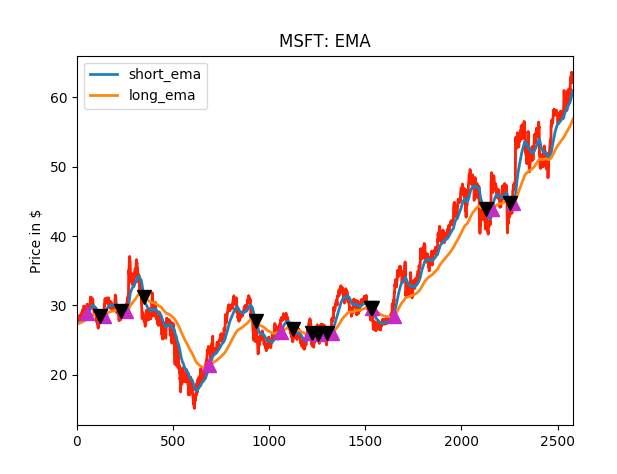
\includegraphics[width=90mm]{EMA_MSFT.png}
\caption{Dual Moving Average Strategy with Exponential effects applied to MSFT \label{overflow}}
\end{figure}

\section*{Analysis}

\subsection*{Effectiveness}
EMA is far more effective at reading recent stock trends that SMA. Because there is little to no lagged effect, we can see the exponential average hug the stock price far closer than SMA in Figure 1. Because of this, we should expect to see buy and sell orders that generate more profit in the long term. 

\subsection*{Runtime}
The components to consider for this strategy include pulling stock data into a Pandas data frame and calculating rolling means from the data-frame and marking their differences. Pandas is a python data analysis package and is perhaps the most powerful open source data analysis or manipulation tool available. For each calculation, it has to scrape through the entire data-frame at a rolling window, giving a linear runtime.

\subsection*{Quality Metric}
The strategy is tested against a baseline long position of 100 shares of a given stock. Therefore, we compare the strategy against simply buying 100 shares of stock right at the opening date and then sell at the final date. For our implementation, over 15 different stocks were chosen and run against this baseline. Unfortunately, most EMA implementations didn't outperform the baseline. However, all EMA's performance did outperform the previously implemented SMA's besides INTC. AAPL nearly doubled it's profit from changing to this exponential windows yet still had 2.53\% less returns than the baseline. GOOG had an over \$10000 positive difference in returns. Interestingly INTC with EMA actually had negative returns while it's SMA had positive. However, there were a couple of instances of lesser performance, such as QCOM, which saw negative profits with EMA while actually greater profits than the baseline with SMA. Overall, the strategy is a massive improvement over the lag prone SMA.

\subsection*{Space / Memory implications}
The only space for SMA required is the data-frame, which is very reasonable.

\section*{Conclusion}
EMA is a massive improvement over SMA in a higher frequency trading situation. Without the lagged effect, we generally see far more returns. However, this basic strategy still doesn't beat the baseline except on a rare occasion. Expectation wise, it is shocking that even basic strategies have yet to outperform the baseline.

\section*{Implementation}
\begin{verbatim}
def execute(stock, start_date, end_date):
    stock = stockDataRetriever(stock, start_date, end_date).getStock()

    # Initialize the short and long windows and buy sell in df
    short_window = 12
    long_window = 26

    # set Pandas df with stock data
    df = pd.DataFrame(index=stock.index)

    # Create short and long simple moving average
    df[short_exponential_moving_average] = df.ema(short_window)
    df[long_exponential_moving_average] = df.ema(long_window)

    # mark signal based on comparison of the two averages
    df[signal] = df.compare(short_exponential_moving_average, long_exponential_moving_average,1,0)

    # when signal changes from 1 to 0 or 0 to 1 - is a buy or sell
    df[positions] = df[signal].diff()

\end{verbatim}

\bibliographystyle{plain}
\bibliography{References}

\end{document}